\chapter{Time Management}

\section{Roadmap}
\begin{figure}[H]
    \centering
    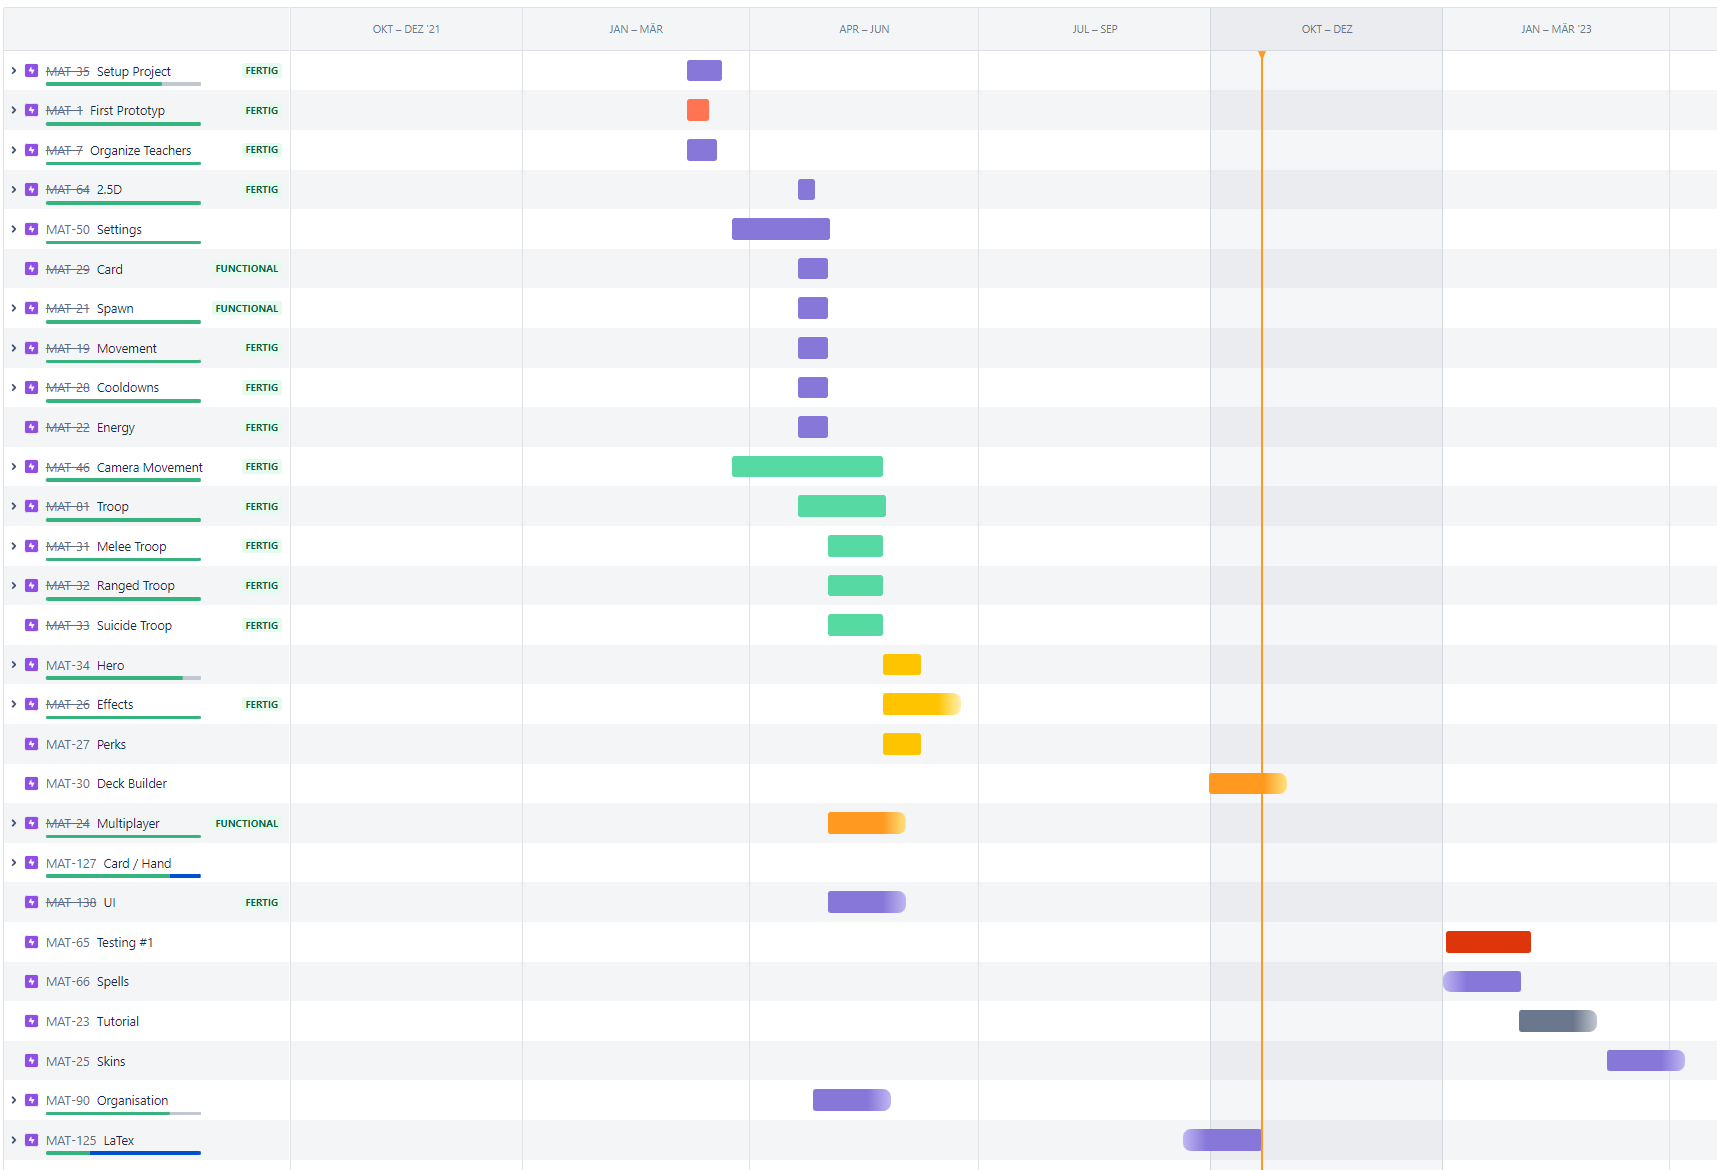
\includegraphics[width=15cm]{resources/roadmap_r.png}\\
    \caption{Roadmap (auf Jira)}
\end{figure}    


\section{Time-Tracking}
\begin{figure}[H]
    \centering
    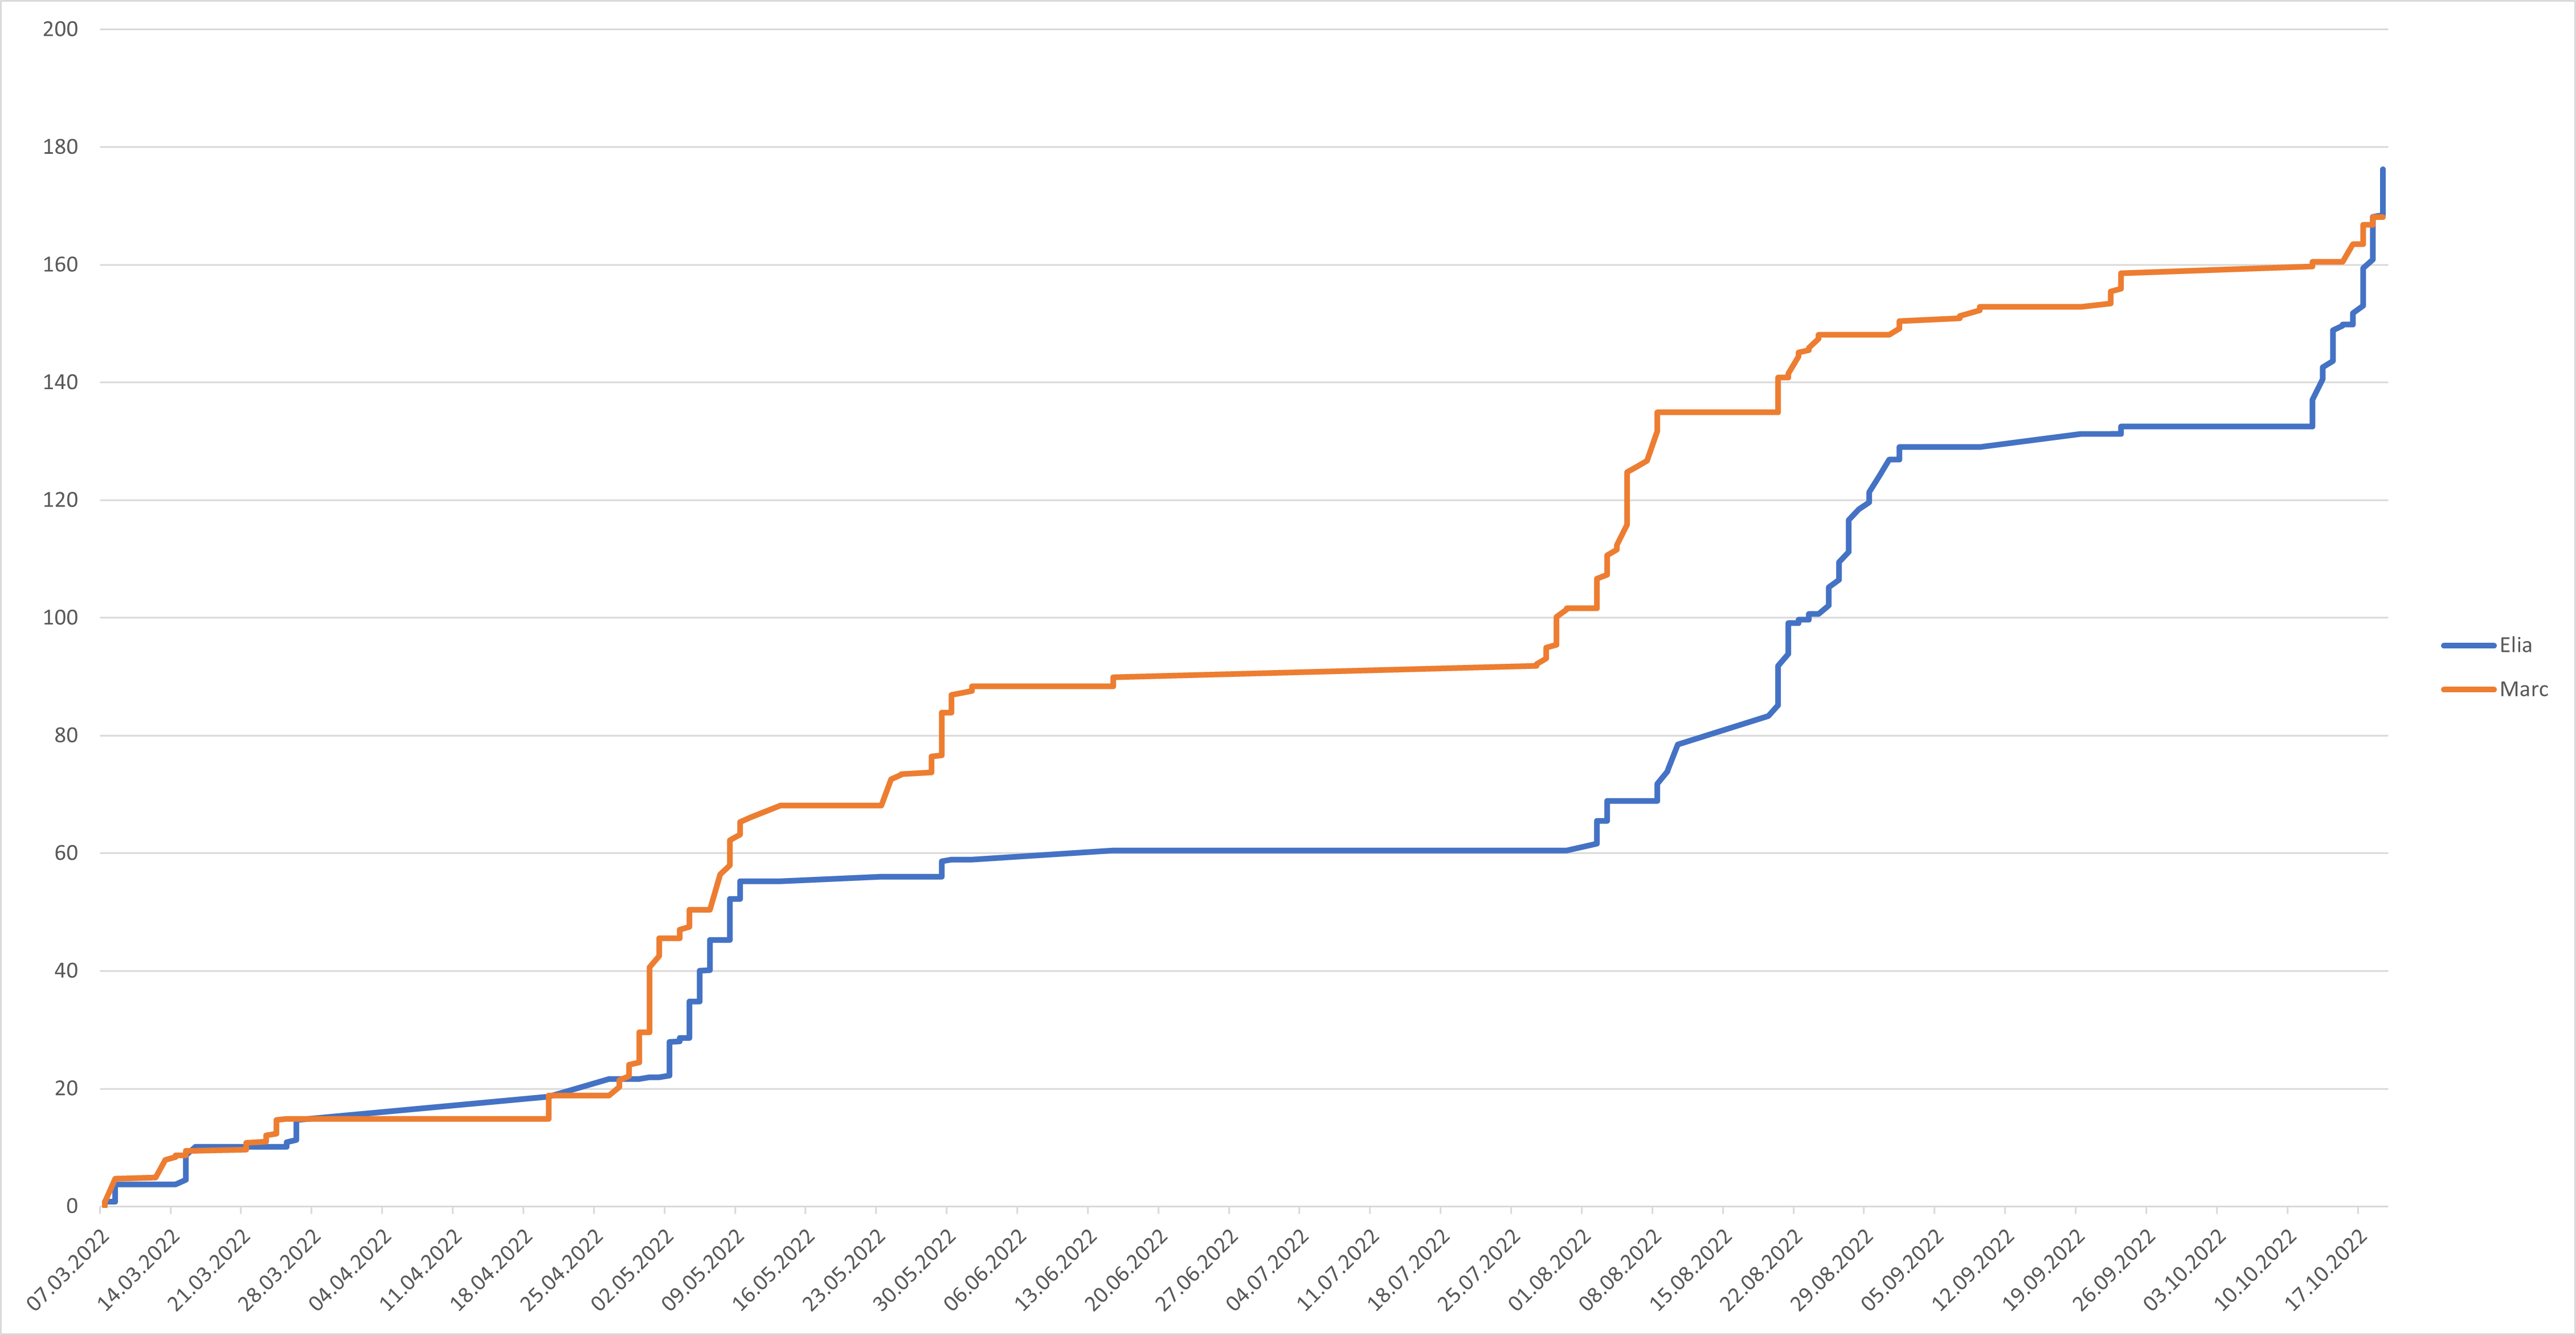
\includegraphics[width=15cm]{resources/graph.png}\\
    \caption{Zeitaufwand seit Beginn der Arbeit}
\end{figure}    

DA NO EXPECTED IN GRAPH (mind und max 100-150)\\
\\
TEAM HOURS mind =120, max =150\\
\\

\begin{figure}[H]
    \centering
    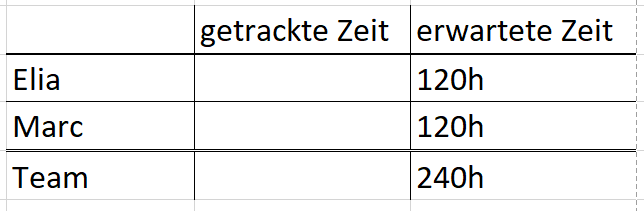
\includegraphics[width=9cm]{resources/tracket_time_temp.png}\\
    \caption{gesamter Zeitaufwand}
\end{figure}



%treffen mit hunzi und jezek oder starbucks oder dihei....
%07.03 treffe mit hunzi im inf büro 45m
%08.03 treffe im starbucks vor em theater 3h
%15.03 jezek und hunzi im 1.03 oder so 45m
%20.04 treffe bim marc vor allem roadmap 4h
%04.05 treffe mit hunzi im besprechigszimmer 2.20 2h
%15.6 treffen mit hunzi im 2.20(gruppenzimmer) nach morgenschuel 1h30m
%01.09 treffe mit hunzi nach vormittagsschuel im 12i 1h20m
%23.09 treffe mit hunzi nach 16h 1h 15m
%16.10 starbucks vor bowle 2h

%genauer am anfang festlegen was genau tracken
